\def\retinanet{
    RetinaNet \cite{lin2017focal} là một mô hình single-stage object detection cân bằng giữa độ chính xác của các mô hình two-stage và tốc độ của các mô hình single-stage ở thời điểm đó.
    Nhóm tác giả của RetinaNet đưa ra vấn đề về các mô hình single-stage như YOLO \cite{redmon2016look} hay SSD \cite{liu2016ssd} dù đạt tốc độ rất nhanh nhưng lại kém các mô hình two-stage một khoảng rất xa về độ chính xác và đề xuất giải pháp khắc phục vấn đề này.

    \noindent
    \textbf{\textit{Tổng quan về các mô hình single-stage object detection}} \\
    Các mô hình single-stage object detection ở thời điểm đó đa phần đều chỉ sử dụng một backbone CNN kết hợp thêm với các lớp Conv và lớp fully connected để đưa ra dự đoán về lớp của đối tượng trong ảnh và độ lệch của bounding box so với groundtruth.
    
    \begin{figure}[H]
        \centering
        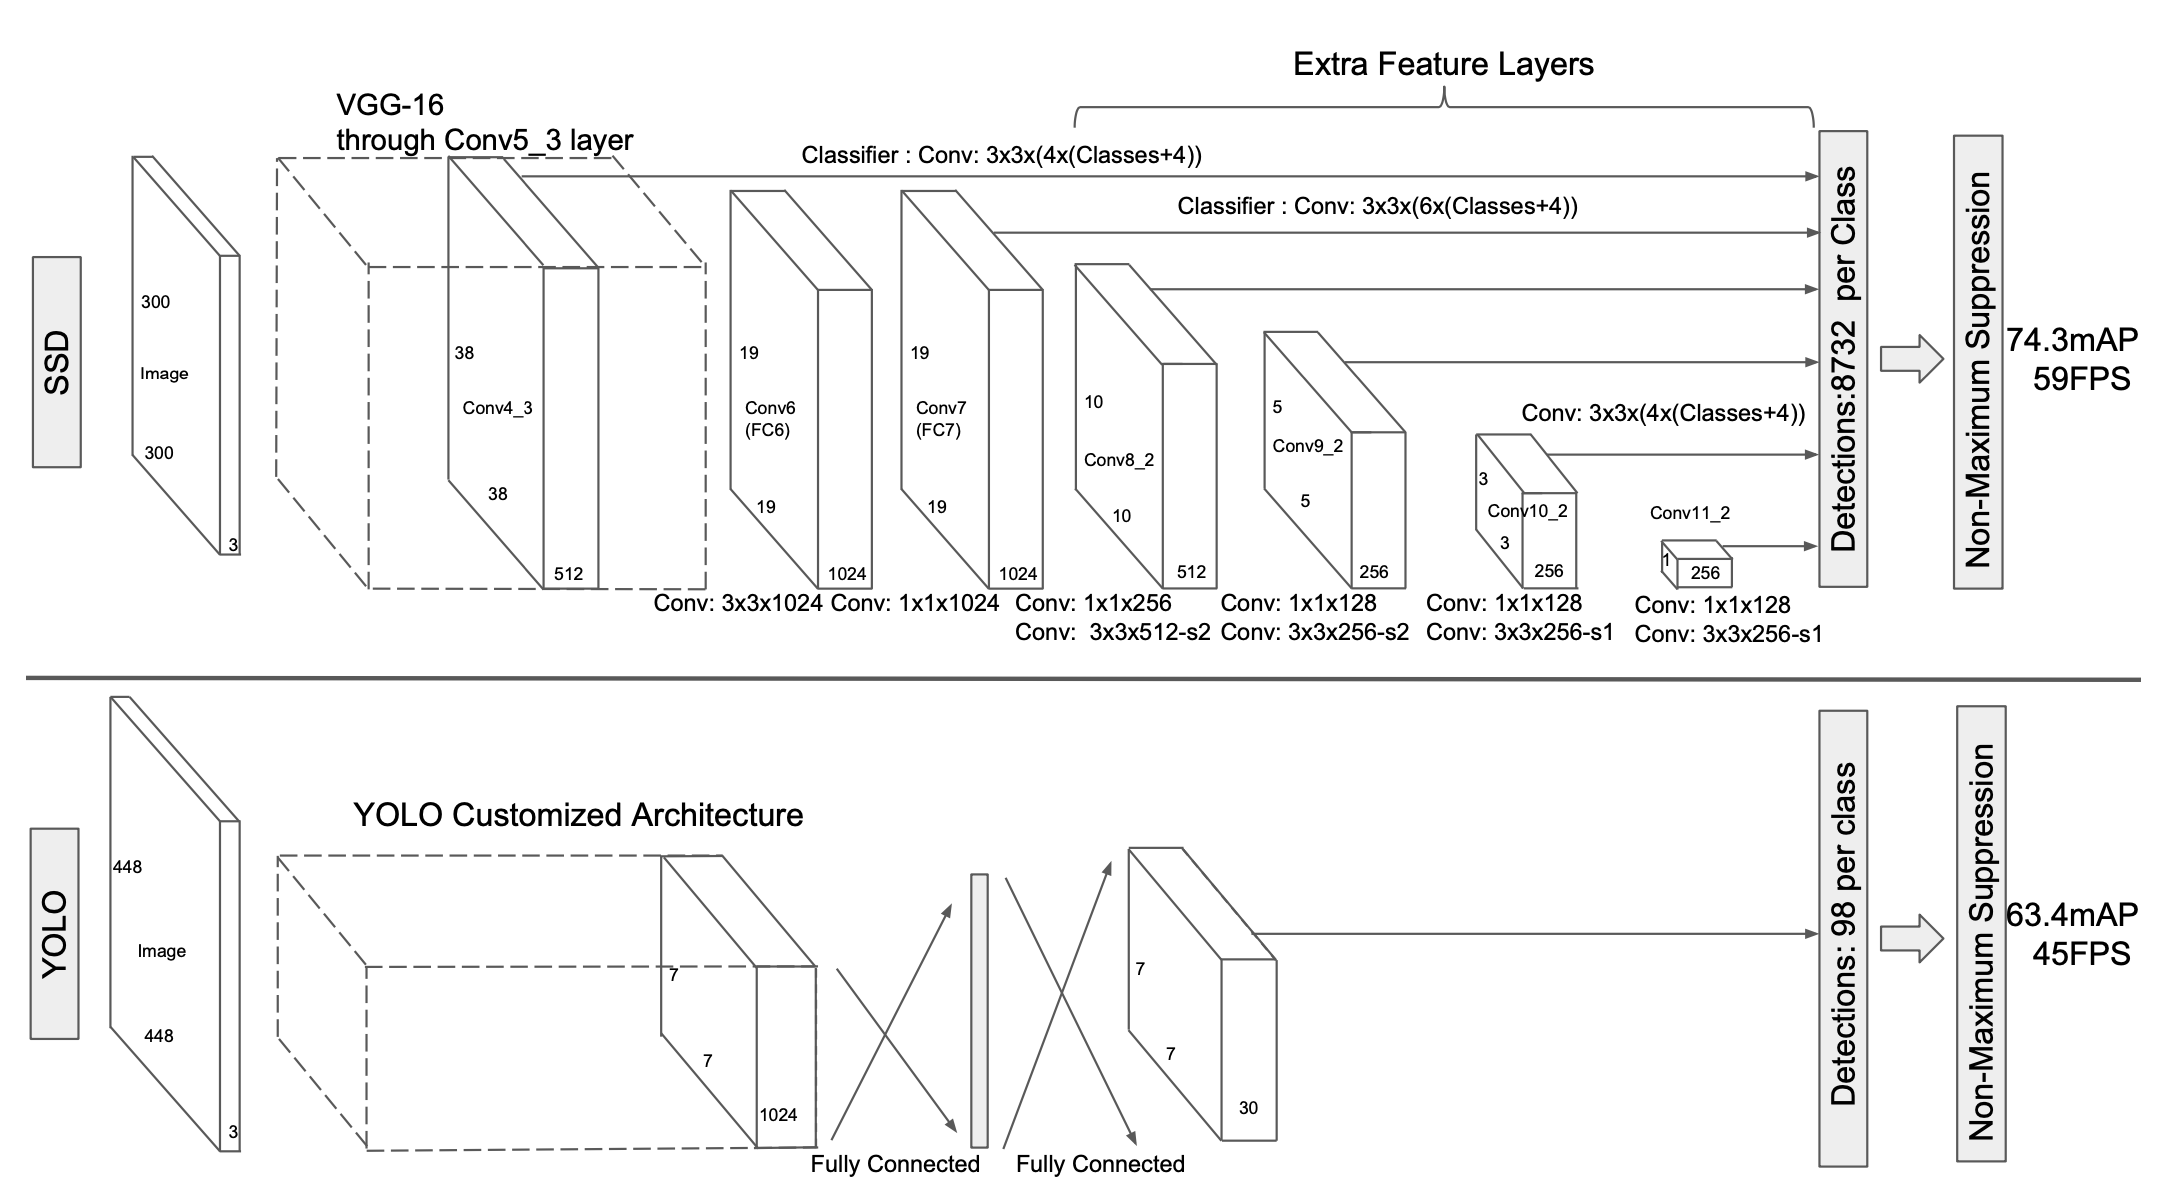
\includegraphics[width=10cm] {images/yolo_ssd_model}
        \caption{Chi tiết hai kiến trúc mô hình single-stage nổi tiếng là SSD và YOLO. (Nguồn: \cite{liu2016ssd})}
        \label{fig:yolo_ssd_model}
    \end{figure}

    \noindent
    Việc loại bỏ Region proposals module khiến các mô hình single-stage object detection cần phải xây dựng một phương pháp riêng nhằm đề xuất ra các anchor chứa đối tượng.
    Hai mô hình single-stage object detection nổi tiếng vào thời điểm đó là YOLO \cite{redmon2016look} và SSD \cite{liu2016ssd} có các cách đề xuất ra anchor tương tự với nhau.
    
    \begin{figure}[H]
        \centering
        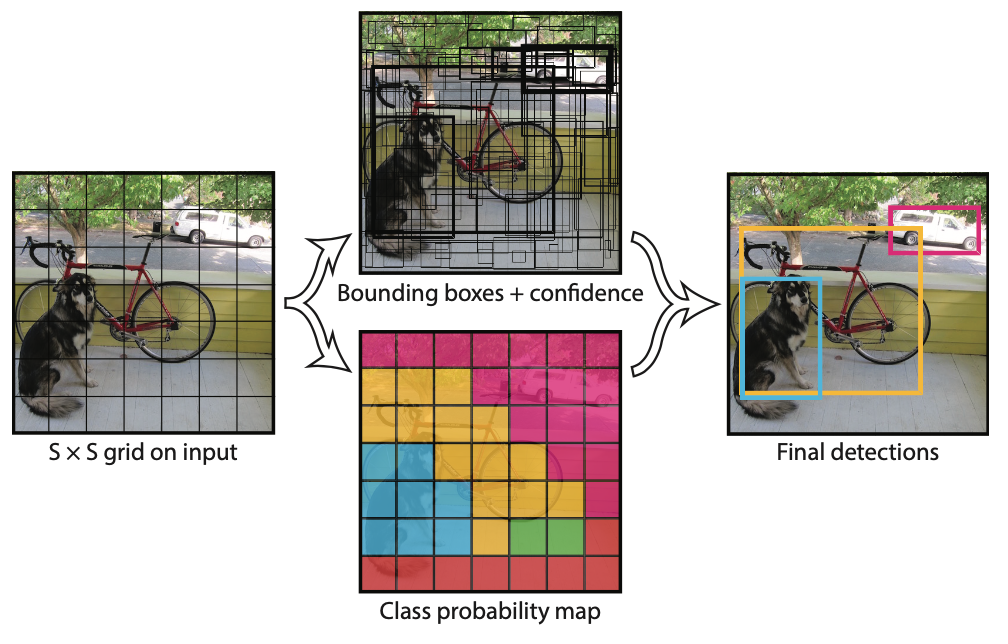
\includegraphics[width=10cm] {images/yolo_anchor}
        \caption{Cách đề xuất anchor của mô hình YOLO. (Nguồn: \cite{redmon2016look})}
        \label{fig:yolo_anchor}
    \end{figure}

    \noindent
    YOLO đề xuất ra các anchor thông qua việc chia ảnh đầu vào thành dạng grid có kích thước $S × S$ và với mỗi grid sẽ trả đầu ra dự đoán có kích thước $S × S × (B * 5 + C)$.
    Nếu tâm của một bounding box nằm trong ô nào trên grid, ô đó sẽ cần phải được dự đoán là chứa đối tượng.
    Mỗi ô trên grid sẽ được mô hình dự đoán $(B * 5 + C)$ giá trị, trong đó: \\
    - B là số lượng bounding box dự đoán. \\
    - 5 là các giá trị trong đó có 4 giá trị x, y, w, h đại diện cho bounding box được dự đoán và 1 giá trị confidence.
    Thay vì được học là 1 nếu anchor có IoU cao với groundtruth bounding box và ngược lại là 0 nếu anchor có IoU thấp với groundtruth bounding box, điểm đặc biệt về giá trị confidence mà nhóm tác giả thiết kế trong mô hình YOLO là nó bằng chính giá trị IoU so với groundtruth. \\
    - C là số lượng lớp đối tượng trong bài toán object detection.
    Mỗi giá trị dự đoán trong C là giá trị xác suất điều kiện nếu ô trên grid chứa đối tượng thì đó là đối tượng nào. \\
    Trong nghiên cứu, nhóm tác giả của YOLO sử dụng $S = 7, B = 2, C = 20$.

    \begin{figure}[H]
        \centering
        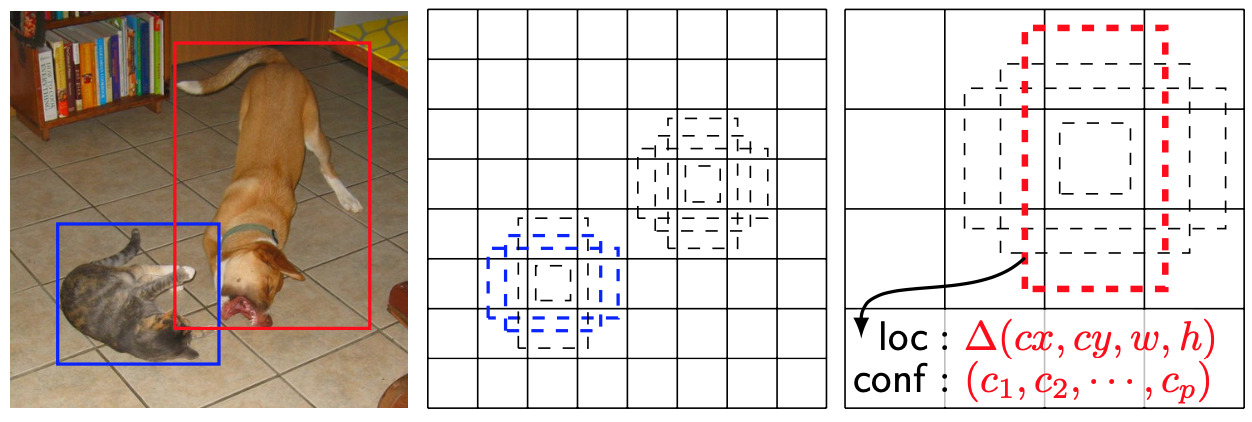
\includegraphics[width=10cm] {images/ssd_anchor}
        \caption{Cách đề xuất anchor của mô hình SSD. (Nguồn: \cite{liu2016ssd})}
        \label{fig:ssd_anchor}
    \end{figure}
    
    \noindent
    SSD cũng sử dụng feature maps như là các dạng grid của ảnh đầu vào nhưng thay vì sử dụng một grid như YOLO thì SSD sử dụng nhiều grid từ nhiều feature maps có cách kích thước khác nhau.
    Với mỗi grid tạo bởi một feature maps có kích thước $m × n$, SSD trả đầu ra dự đoán có kích thước $m × n × (k × (c + 4))$.
    Nếu tâm của một bounding box nằm trong ô nào trên grid, ô đó sẽ cần phải được dự đoán là chứa đối tượng.
    Mỗi ô trên grid sẽ được mô hình dự đoán $(k × (c + 4))$ giá trị, trong đó: \\
    - k là số lượng bounding box dự đoán. \\
    - 4 là 4 giá trị x, y, w, h đại diện cho bounding box được dự đoán. \\
    - c là số lượng lớp đối tượng trong bài toán object detection.
    Mỗi giá trị dự đoán trong c là giá trị xác suất anchor đó là đối tượng nào.

    \noindent
    Với ý tưởng khởi tạo anchor như trên, nhóm tác giả của RetinaNet đã chỉ ra một vấn đề nghiêm trọng mà các mô hình single stage object detection nói chung gặp phải đó là vấn đề mất cân bằng dữ liệu trong quá trình train mô hình.
    Cụ thể, vấn đề mất cân bằng ở đây xảy ra chủ yếu do sự chênh lệch giữa phần ảnh là foreground và phần ảnh là background, hay nói cách khác là phần ảnh chứa đối tượng và phần ảnh không chứa đối tượng. \\
    Các mô hình two-stage object detection không thật sự gặp phải vấn đề mất cân bằng dữ liệu này bởi vì trong quá trình đưa các khu vực đề xuất từ Region proposals module sang Feature extraction module thường đã có một bước lọc và lựa chọn.
    Cụ thể hơn, với số lượng lớn các khu vực không chứa đối tượng được đề xuất bởi Region proposals module, chỉ có một số ít trong đó được lựa chọn để làm đầu vào cho Feature extraction module và lúc này, tỷ lệ giữa các khu vực chứa và không chứa đối tượng thường là 1:3 - một tỷ lệ mất cân bằng không quá nghiêm trọng và không ảnh hưởng tới việc train mô hình object detection.

    \noindent
    \textbf{\textit{Hàm Focal loss}} \\
    Để giải quyết vấn đề mất cân bằng dữ liệu nói trên, nhóm tác giả của RetinaNet đã đề xuất hàm Focal loss dựa trên nền tảng của hàm binary cross entropy loss giải quyết vấn đề mất cân bằng dữ liệu nghiêm trọng.
    Nhóm tác giả chú thích rằng hàm Focal loss hiệu quả đối với cả bài toán phân lớp với nhiều hơn hai lớp nhưng để đơn giản hoá, nhóm tác giả sử dụng hàm binary cross entropy loss.

    \begin{equation}
        \label{eq:bce}
        CE(p,y) = 
        \begin{cases}
            -\log(p) &\text{if $y = 1$} \\
            -\log (1 - p) &\text{otherwise.}
        \end{cases}
    \end{equation}

    \noindent
    trong đó: \\
    - y là giá trị groundtruth (0 đối với anchor không chứa object và 1 đối với anchor chứa object) \\
    - p là giá trị xác suất mà mô hình dự đoán anchor đó chứa object \\
    Để ngắn gọn, nhóm tác giả quy ước lại như sau:

    \begin{equation}
        \label{eq:bce}
        p_\textrm{t} =
        \begin{cases}
            p &\text{if $y = 1$} \\
            1 - p &\text{otherwise,}
        \end{cases}
    \end{equation}

    \noindent
    từ đó, hàm cross entropy loss được viết lại thành

    \begin{equation}
        CE(p,y) = CE(p_\textrm{t}) = - \log (p_\textrm{t})
    \end{equation}

    \noindent
    Một cấu hình khác của hàm cross entropy loss là \textit{balanced cross entropy loss}, được sinh ra bằng việc đánh trọng số cho từng số hạng của hàm cross entropy loss ban đầu

    \begin{equation}
        CE(p,y) = - \alpha_\textrm{t} \log (p_\textrm{t})
    \end{equation}

    \noindent
    trong đó: \\
    - $\alpha_\textrm{t}$ là trọng số tương ứng với số hạng $p_\textrm{t}$.
    Trọng số $\alpha_\textrm{t}$ có thể được tính dựa trên tần suất xuất hiện của các lớp trong bộ dữ liệu hoặc là một hyperpameter.

    \noindent
    Hàm balanced cross entropy loss có thể đã giúp giảm bớt hiệu ứng mất cân bằng dữ liệu lên trên giá trị hàm loss.
    Tuy nhiên, việc gán trọng số như hàm balanced cross entropy loss không phân biệt được giữa những mẫu dữ liệu dễ và khó.
    Nhóm tác giả, từ đó, đề xuất hàm \textit{Focal loss} không những giúp giải quyết vấn đề mất cân bằng dữ liệu mà còn giúp mô hình tập trung vào những mẫu dữ liệu \textit{không chứa đối tượng} nhưng khó và dễ nhầm lẫn thành \textit{chứa đối tượng}.

    \begin{equation}
        FL(p_\textrm{t}) = - (1 - p_\textrm{t})^\gamma \log (p_\textrm{t})
    \end{equation}

    \noindent
    trong đó: \\
    - $(1 - p_\textrm{t})$ là thành phần đánh giá độ dễ hay khó của mẫu dữ liệu.
    Với những mẫu dễ và mô hình đã được train tốt, giá trị $(1 - p_\textrm{t})$ sẽ nhỏ và những mẫu này sẽ gây ít ảnh hưởng trong quá trình train mô hình. \\
    - $\gamma$ được nhóm tác giả gọi là \textit{focusing parameter}, dùng để xác định mức độ tập trung của mô hình lên các mẫu dữ liệu không chứa đối tượng.
    Với $\gamma = 0$, hàm FL lúc này tương tự với hàm CE.
    Trong các thí nghiệm của RetinaNet, giá trị $\gamma = 2$ là tốt nhất.

    \begin{figure}[H]
        \centering
        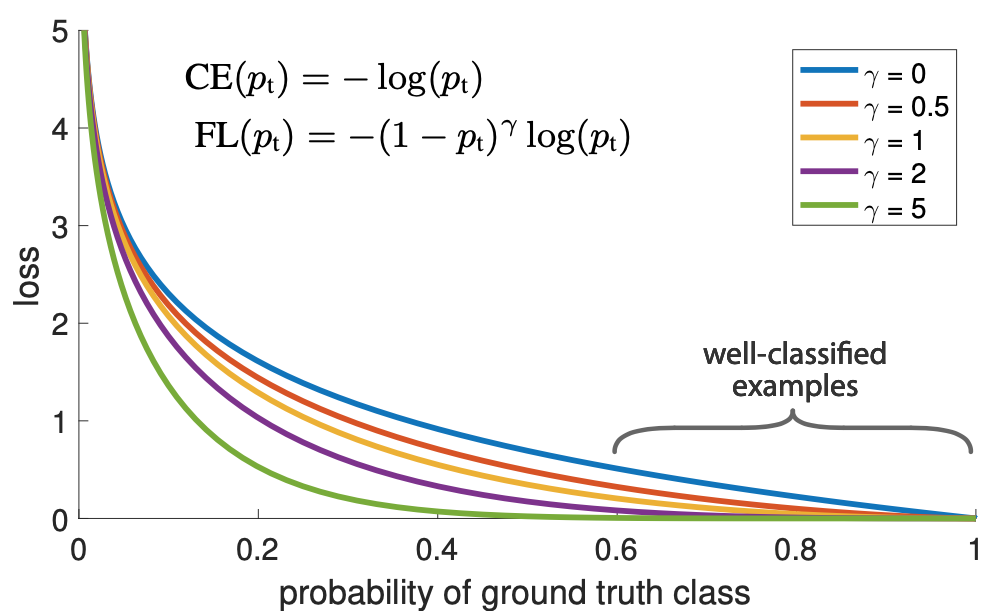
\includegraphics[width=10cm] {images/retinanet_focal_loss_curve}
        \caption{So sánh các tham số của hàm Focal loss với hàm Cross Entropy loss. (Nguồn: \cite{lin2017focal})}
        \label{fig:retinanet_focal_loss_curve}
    \end{figure}

    \noindent
    Ngoài ra, nhóm tác giả còn đề xuất một dạng khác của hàm FL bằng việc sử dụng thêm một tham số $\alpha$ và trong các thí nghiệm, dạng này cho kết quả tốt hơn một chút so với dạng hàm FL không sử dụng $\alpha$.

    \begin{equation}
        FL(p_\textrm{t}) = - \alpha_\textrm{t} (1 - p_\textrm{t})^\gamma \log (p_\textrm{t})
    \end{equation}
    
    \noindent
    \textbf{\textit{Kiến trúc mô hình RetinaNet}} \\
    RetinaNet là mô hình single-stage object detection gồm có các thành phần:
    - Phần \textit{backbone Feature Pyramid Networks} được sử dụng nhằm trích xuất đặc trưng của ảnh đầu vào với nhiều kích thước đặc trưng khác nhau.
    Chi tiết về sức mạnh của FPN đã được thảo luận ở \textit{phần 2.2. Kiến trúc Feature Pyramid Networks}.
    - Phần trích xuất anchor được thực hiện tương tự với cách trích xuất của mô hình RPN biến thể đã phân tích ở \textit{phần 2.2}.
    Tuy nhiên, nhóm tác giả đã thử nghiệm và bổ sung thêm các kích thước $2^{0}$, $2^{1/3}$, $2^{2/3}$ của anchor để đạt kết quả tốt hơn.
    Các anchor được gán groundtruth với chiến lược tương tự như trong \textit{phần 2.1.3. Mô hình Faster R-CNN} nhưng điều chỉnh một số điểm: (1) thay đổi trở thành bài toán multi-class classification (nhóm tác giả của \textit{phần 2.1.3} sử dụng bài toán binary classification phân lớp giữa \textit{anchor có chứa object} và \textit{anchor không chứa object}) và (2) thay đổi threshold IoU để gán nhãn cho từng anchor.

    \begin{figure}[H]
        \centering
        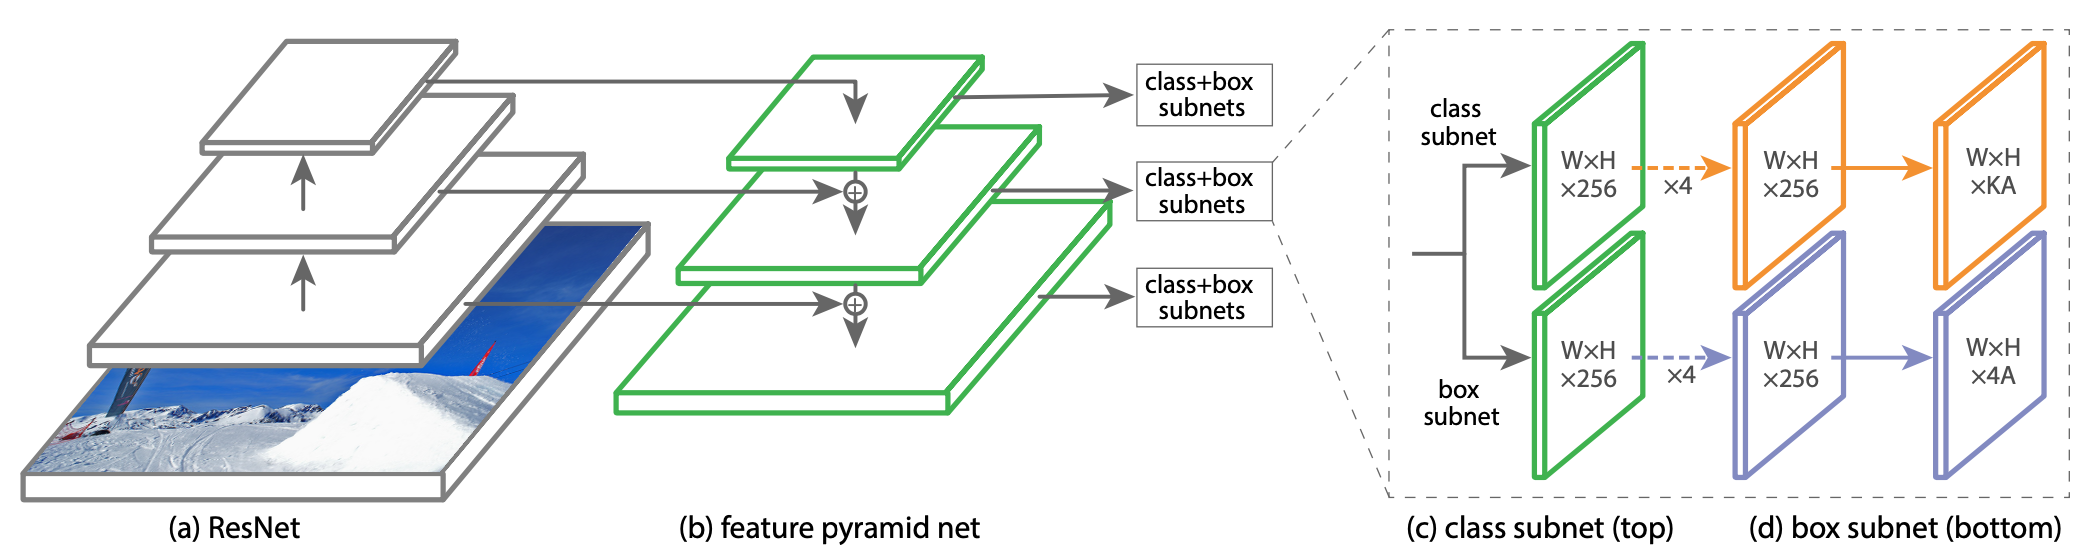
\includegraphics[width=10cm] {images/retinanet_model}
        \caption{Kiến trúc mô hình RetinaNet. (Nguồn: \cite{lin2017focal})}
        \label{fig:retinanet_model}
    \end{figure}

    \noindent
    - Phần \textit{Classification Subnet} được chia sẻ giữa tất cả các feature maps của backbone FPN, gồm các lớp Conv 3x3xC và lớp Conv cuối cùng 3x3xKA.
    Trong đó, K là số lượng lớp đối tượng trong bài toán object detection, A là số lượng anchor tại vị trí trên mỗi feature maps của backbone FPN (tác giả chọn $A = 9$), C là số lượng channel của lớp Conv (tác giả chọn $C = 256$). \\
    - Phần \textit{Box Regression Subnet} được thiết kế khác với cách thiết kế trong mô hình Faster R-CNN khi không dùng chung các lớp Conv với \textit{Classification Subnet}.
    \textit{Box Regression Subnet} cũng gồm các lớp Conv 3x3xC và lớp Conv cuối cùng 3x3x4A.
    Trong đó, A là số lượng anchor tại vị trí trên mỗi feature maps của backbone FPN (tác giả chọn $A = 9$), 4 là 4 độ lệch trong toạ độ của bounding box dự đoán so với groundtruth, C là số lượng channel của lớp Conv (tác giả chọn $C = 256$).

    \noindent
    \textbf{\textit{Kết quả của mô hình RetinaNet}} \\
    Trong thử nghiệm của RetinaNet với các tham số khác nhau của hàm Focal loss, tất cả các cấu hình được train với bộ dữ liệu \textit{COCO trainval135k} và kết quả thu được đánh giá trên bộ dữ liệu \textit{COCO minival}.
    Kết quả của cấu hình $\gamma = 2.0$ và $\alpha = 0.25$ đạt kết quả tốt nhất so với các cấu hình khác của hàm Focal loss.

    \begin{figure}[H]
        \centering
        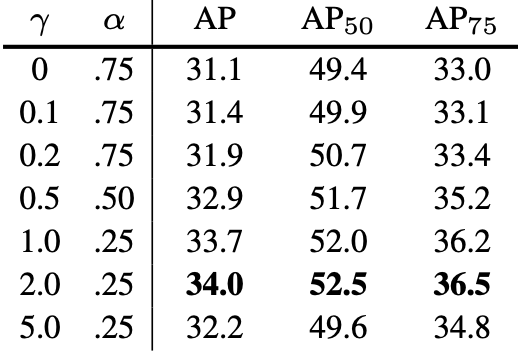
\includegraphics[width=10cm] {images/retinanet_results_2}
        \caption{Kết quả thử nghiệm hàm Focal loss với các tham số khác nhau. (Nguồn: \cite{lin2017focal})}
        \label{fig:retinanet_results_2}
    \end{figure}

    Khi so sánh kết quả của mô hình RetinaNet với các mô hình object detection khác vào thời điểm đó, kết quả của các cấu hình khác nhau của mô hình RetinaNet cũng đạt kết quả rất tốt về cả tốc độ lẫn độ chính xác của mô hình.
    Cụ thể các mô hình được so sánh gồm: \\
    - Kết quả của mô hình YOLOv2 ký hiệu là [A] \cite{redmon2016yolo9000} (Kết quả không được biểu diễn trên hình) \\
    - Kết quả của mô hình SSD321, ký hiệu là [B] \cite{liu2016ssd} \\
    - Kết quả của mô hình DSSD321, ký hiệu là [C] \cite{fu2017dssd} \\
    - Kết quả của mô hình R-FCN, ký hiệu là [D] \cite{dai2016r} \\
    - Kết quả của mô hình SSD513, ký hiệu là [E] \cite{liu2016ssd} \\
    - Kết quả của mô hình DSSD513, ký hiệu là [F] \cite{fu2017dssd} \\
    - Kết quả của mô hình FPN FRCN, ký hiệu là [G] \cite{lin2017feature} \\
    - Kết quả của mô hình RetinaNet sử dụng backbone là ResNet50 và sử dụng ảnh đầu vào có kích thước 500 pixel, ký hiệu là RetinaNet-50-500. \\
    - Kết quả của mô hình RetinaNet sử dụng backbone là ResNet101 và sử dụng ảnh đầu vào có kích thước 500 pixel, ký hiệu là RetinaNet-101-500 \\
    - Kết quả của mô hình RetinaNet sử dụng backbone là ResNet101 và sử dụng ảnh đầu vào có kích thước 800 pixel, ký hiệu là RetinaNet-101-800 \\
    Đường màu xanh và màu cam trên hình lần lượt là các cấu hình RetinaNet sử dụng backbone ResNet50 và ResNet101 và với các cấu hình ảnh đầu vào từ 400 pixel đến 800 pixel.

    \begin{figure}[H]
        \centering
        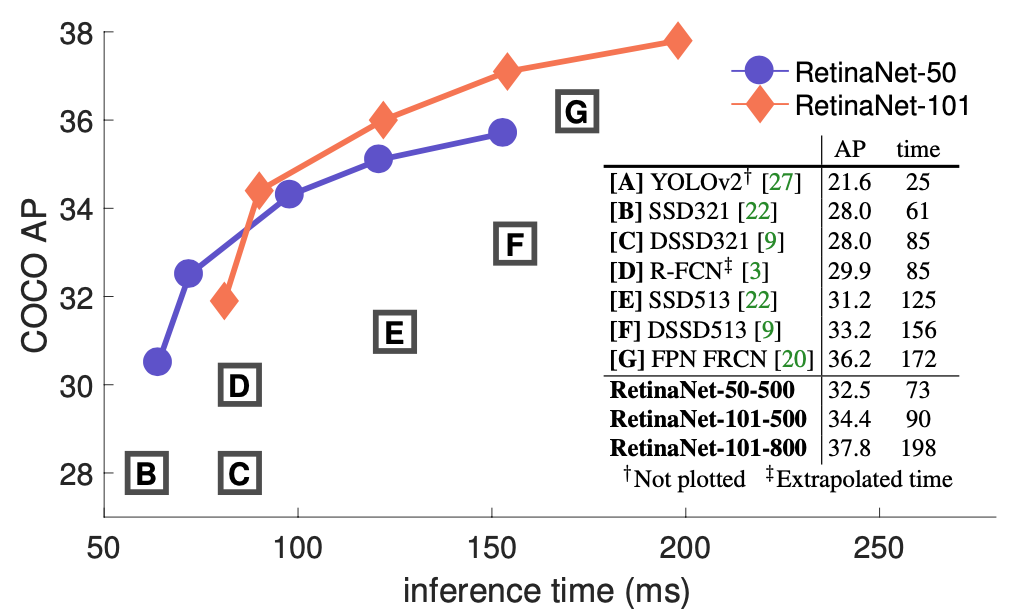
\includegraphics[width=6cm] {images/retinanet_results_1}
        \caption{So sánh kết quả mô hình RetinaNet với một số mô hình object detection khác. (Nguồn: \cite{lin2017focal})}
        \label{fig:retinanet_results_1}
    \end{figure}

    Kết quả, các cấu hình khác nhau của RetinaNet đều cho kết quả tốt hơn so với các mô hình object detection khác (cả single-stage và two-stage).
    So với mô hình đạt độ chính xác tốt nhất ở thời điểm đó là [G], cấu hình RetinaNet-101-700 cho kết quả chính xác hơn với thời gian nhanh hơn.
    So với các mô hình đạt tốc độ tốt nhất ở thời điểm đó là [A] và [B], cấu hình RetinaNet-50-400 cho kết quả chậm hơn nhưng với độ chính xác cao hơn vượt trội.

    \noindent
    \textbf{\textit{Kết luận về mô hình RetinaNet}} \\
    Mô hình RetinaNet ra đời là một bước tiến lớn đối với việc giải quyết bài toán object detection khi nó giải quyết vấn đề mất cân bằng dữ liệu của các mô hình single-stage giúp tăng độ chính xác của mô hình ngang bằng với các mô hình two-stage nhưng vẫn duy trì được một tốc độ nhanh và có thể sử dụng trong thời gian thực. \\
    Mô hình RetinaNet cho đến nay vẫn là một mô hình tốt để giải quyết các bài toán con của object detection, cụ thể là face detection.
    Trong các phần tiếp theo của luận văn, ta sẽ bàn luận về các mô hình kế thừa RetinaNet giải quyết rất tốt bài toán face detection.
}